% chapters/07-local-network.tex

\chapter{Building Your Local Network}\label{ch:building-your-local-network}

\begin{importantbox}
I've watched talented entrepreneurs struggle in Nigeria, not because they lacked capability, but because they lacked connections. Let me share what I've learned about building the right networks in the right way.
\end{importantbox}

\section{The Network Effect: Beyond Business Cards}\label{sec:network-effect}

When I first started working within Lagos, I made what I call the ``Silicon Valley mistake'' --- thinking I could build relationships the same way I did in tech hubs.\ I quickly learned that Nigerian business networks operate differently.

\begin{tcolorbox}[colback=white,colframe=primarydark,title=\textbf{Network Building Principles}]
\begin{itemize}
    \item \textbf{Personal Before Professional}
    Begin relationships with genuine personal connection before business

    \item \textbf{Respect the Hierarchy}
    Understand and acknowledge traditional business structures

    \item \textbf{Value Exchange First}
    Lead with what you can offer before asking for anything

    \item \textbf{Long-term View}
    Build relationships for the future, not just immediate needs
\end{itemize}
\end{tcolorbox}

\section{Strategic Network Mapping}\label{sec:strategic-network-mapping}

Let me share what I call the ``Five Circles Framework'' --- a strategic approach to building your Nigerian business network:

\begin{figure}[h]
    \centering
    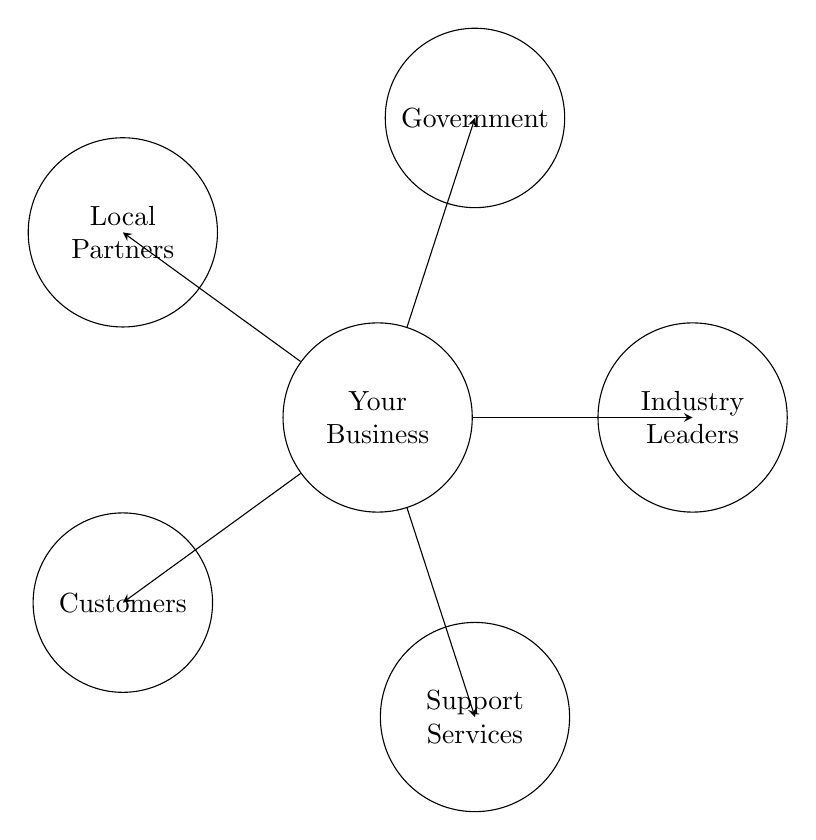
\begin{tikzpicture}[node distance=2cm]
        % Core circle
        \node[draw, circle, text width=2cm, align=center] (core) {Your\\Business};

        % Surrounding circles with key relationships
        \foreach \angle/\label in {
            0/Industry Leaders,
            72/Government,
            144/Local Partners,
            216/Customers,
            288/Support Services
        } {
            \node[draw, circle, text width=2cm, align=center]
                at (\angle:4) {\label};
            \draw[-stealth] (core) -- (\angle:4);
        }
    \end{tikzpicture}
    \caption{The Five Circles Network Framework}
    \label{fig:five-circles}
\end{figure}

\section{Regional Network Development}\label{sec:regional-network-development}

\begin{regionalbox}{United Kingdom}
For UK entrepreneurs, especially in financial services:

\begin{itemize}
    \item \textbf{Primary Networks}
    \begin{itemize}
        \item Nigeria-British Chamber of Commerce
        \item UK-Nigeria Financial Services Working Group
        \item Commonwealth Business Network
    \end{itemize}

    \item \textbf{Key Events}
    \begin{itemize}
        \item Annual Nigeria Banking Conference
        \item UK-Nigeria Investment Summit
        \item Commonwealth Business Forum
    \end{itemize}

    \item \textbf{Strategic Partnerships}
    \begin{itemize}
        \item Local banking institutions
        \item Financial regulatory bodies
        \item Professional service firms
    \end{itemize}
\end{itemize}
\end{regionalbox}

\begin{regionalbox}{United States}
For US tech entrepreneurs:

\begin{itemize}
    \item \textbf{Tech Ecosystem Access}
    \begin{itemize}
        \item Lagos Startup Hub
        \item Nigerian Computer Society
        \item American Business Council
    \end{itemize}

    \item \textbf{Innovation Networks}
    \begin{itemize}
        \item Local tech incubators
        \item Developer communities
        \item Industry associations
    \end{itemize}

    \item \textbf{Knowledge Transfer}
    \begin{itemize}
        \item Technical universities
        \item Research institutions
        \item Training centers
    \end{itemize}
\end{itemize}
\end{regionalbox}

\begin{regionalbox}{UAE}
For UAE trade specialists:

\begin{itemize}
    \item \textbf{Trade Networks}
    \begin{itemize}
        \item Nigerian-Arabian Gulf Chamber
        \item Import/Export Associations
        \item Logistics Networks
    \end{itemize}

    \item \textbf{Business Forums}
    \begin{itemize}
        \item UAE-Nigeria Business Forum
        \item Trade Exhibitions
        \item Industry Conferences
    \end{itemize}

    \item \textbf{Government Relations}
    \begin{itemize}
        \item Trade ministries
        \item Customs authorities
        \item Port administrations
    \end{itemize}
\end{itemize}
\end{regionalbox}

\begin{regionalbox}{Canada}
For Canadian sector specialists:

\begin{itemize}
    \item \textbf{Industry Networks}
    \begin{itemize}
        \item Agricultural Associations
        \item Clean Technology Groups
        \item Educational Networks
    \end{itemize}

    \item \textbf{Research Partnerships}
    \begin{itemize}
        \item Universities
        \item Research Institutes
        \item Innovation Centers
    \end{itemize}

    \item \textbf{Government Relations}
    \begin{itemize}
        \item Canadian Trade Commission
        \item Sector Regulators
        \item Industry Bodies
    \end{itemize}
\end{itemize}
\end{regionalbox}

\section{Network Building Timeline}\label{sec:network-building-timeline}

I always tell entrepreneurs to follow what I call the ``Trust Building Timeline'':

\begin{center}
\begin{tabularx}{\textwidth}{>{\raggedright\arraybackslash}X >{\centering\arraybackslash}X >{\raggedright\arraybackslash}X}
    \toprule
    \textbf{Phase} & \textbf{Duration} & \textbf{Focus Areas} \\
    \midrule
    Introduction & 1-2 months & Initial connections and presence \\
    Development & 2-3 months & Relationship deepening \\
    Engagement & 3-6 months & Active collaboration \\
    Integration & 6+ months & Long-term partnerships \\
    \bottomrule
\end{tabularx}
\end{center}

\section{Digital Network Management}\label{sec:digital-network-management}

Modern Nigerian networking requires both traditional and digital approaches:

\begin{tcolorbox}[colback=white,colframe=primarydark,title=\textbf{Digital Networking Tools}]
\begin{itemize}
    \item \textbf{Professional Platforms}
    \begin{itemize}
        \item LinkedIn for professional presence
        \item WhatsApp for business groups
        \item Industry-specific platforms
    \end{itemize}

    \item \textbf{Content Sharing}
    \begin{itemize}
        \item Industry insights
        \item Company updates
        \item Market analysis
    \end{itemize}

    \item \textbf{Community Engagement}
    \begin{itemize}
        \item Online forums
        \item Virtual events
        \item Digital roundtables
    \end{itemize}
\end{itemize}
\end{tcolorbox}

\section{Network Maintenance Strategy}\label{sec:network-maintenance}

Maintaining networks is as important as building them. Here's my ``CARES'' framework:

\begin{itemize}
    \item \textbf{Consistent Communication}
    Regular, meaningful touchpoints

    \item \textbf{Active Participation}
    Regular involvement in network activities

    \item \textbf{Resource Sharing}
    Contributing valuable information and opportunities

    \item \textbf{Event Engagement}
    Attending and hosting key industry events

    \item \textbf{Strategic Support}
    Providing and requesting assistance appropriately
\end{itemize}

\section{Common Networking Mistakes}\label{sec:common-mistakes}

Let me share what I call the ``Four Fatal Flaws'' in Nigerian networking:

\begin{tcolorbox}[colback=white,colframe=primarydark,title=\textbf{Networking Pitfalls}]
\begin{enumerate}
    \item \textbf{The Transactional Trap}
    Focusing only on immediate business needs

    \item \textbf{The Cultural Blind Spot}
    Ignoring local business customs

    \item \textbf{The Digital Dependence}
    Over-relying on online networking

    \item \textbf{The Status Mistake}
    Misunderstanding hierarchical relationships
\end{enumerate}
\end{tcolorbox}

\section{Workshop: Your Network Strategy}\label{sec:network-strategy-workshop}

\begin{workshopbox}
\textbf{Network Development Exercise}

1. Network Mapping
\begin{itemize}
    \item Primary network targets: \_\_\_\_\_\_\_\_\_
    \item Secondary connections: \_\_\_\_\_\_\_\_\_
    \item Resource requirements: \_\_\_\_\_\_\_\_\_
\end{itemize}

2. Relationship Building
\begin{itemize}
    \item Key events to attend: \_\_\_\_\_\_\_\_\_
    \item Value proposition: \_\_\_\_\_\_\_\_\_
    \item Communication strategy: \_\_\_\_\_\_\_\_\_
\end{itemize}

3. Network Maintenance
\begin{itemize}
    \item Regular touchpoints: \_\_\_\_\_\_\_\_\_
    \item Engagement activities: \_\_\_\_\_\_\_\_\_
    \item Resource sharing plan: \_\_\_\_\_\_\_\_\_
\end{itemize}
\end{workshopbox}

\begin{communitybox}
Connect with fellow entrepreneurs and access additional resources on the Africa Growth Circle:
\begin{itemize}
    \item Network directory
    \item Event calendar
    \item Industry forums
    \item Expert connections
    \item Networking guides
\end{itemize}
Visit circle.counseal.com to join the conversation.
\end{communitybox}

\begin{importantbox}
Remember, in Nigeria, your network is not just your net worth --- it's your pathway to sustainable success. In Chapter 8, we'll explore how to leverage these networks in your day-to-day operations.
\end{importantbox}